\section{Phân tích hệ thống}
Chương này trình bày quá trình phân tích hệ thống của đề tài nhằm làm rõ các chức năng,
luồng xử lý và cấu trúc của hệ thống thông qua các mô hình phân tích chuẩn trong kỹ thuật
phần mềm. Dựa trên các yêu cầu chức năng và phi chức năng đã được xác định ở chương
trước, hệ thống được mô hình hóa bằng các Use case Diagram, Activity Diagram, Sequence Diagram và Class Diagram.

Các sơ đồ này giúp mô tả một cách trực quan mối quan hệ giữa người dùng và hệ thống,
các luồng xử lý nghiệp vụ chính, trình tự tương tác giữa các thành phần, cũng như cấu trúc
dữ liệu và mối quan hệ giữa các lớp trong hệ thống. Qua đó, chương này đóng vai trò là cơ
sở cho việc thiết kế và triển khai hệ thống ở các giai đoạn tiếp theo.
\subsection{Use case Diagram }
Hình 4.1 là use case tổng quan của hệ thống được sử dụng để mô tả các chức năng chính của hệ thống và mối quan hệ
giữa các tác nhân (actors) với hệ thống.
\begin{figure}[H]
    \centering
    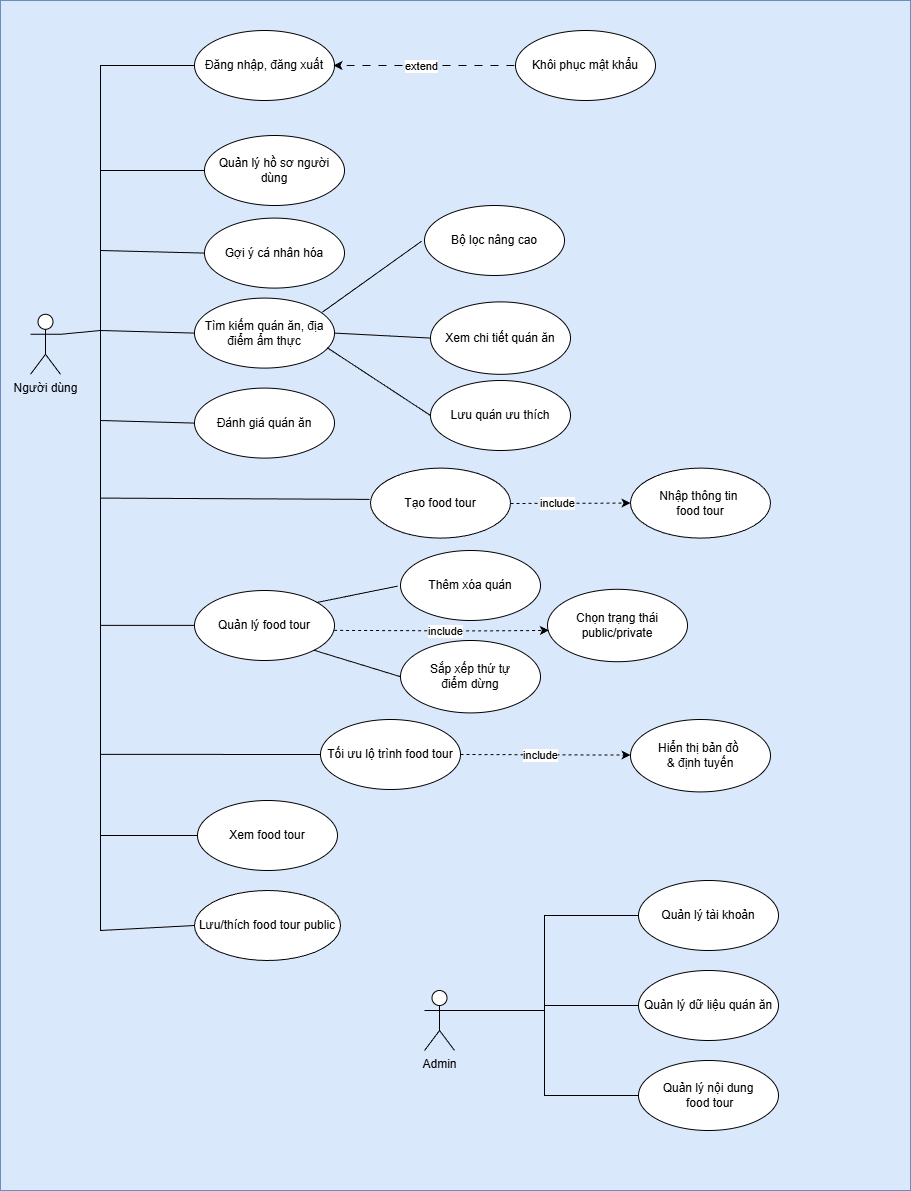
\includegraphics[width=1\linewidth]{img/1.png}
    \caption{Use Case tổng quan}
\end{figure}

\newpage

\subsection{Đặc tả Usecase (Usecase Detail)}

% ==== Đăng nhập, đăng xuất ====
\subsubsection{Usecase: Đăng nhập, đăng xuất}
\begin{longtable}{|p{4cm}|p{10cm}|}
\caption{Usecase: Đăng nhập, đăng xuất}
\\
\hline
\endfirsthead

\hline

\endhead

\hline
\multicolumn{2}{r}{Tiếp trang} \\
\endfoot

\hline
\endlastfoot
\textbf{Usecase name} & Đăng nhập, đăng xuất \\ \hline
\textbf{Description} & Hệ thống cho phép người dùng đăng nhập để truy cập hệ thống và đăng xuất khi kết thúc phiên. \\ \hline
\textbf{Actors} & Người dùng \\ \hline
\textbf{Trigger} & Người dùng chọn chức năng đăng nhập \\ \hline
\textbf{Preconditions} & Người dùng đã có tài khoản hợp lệ \\ \hline
\textbf{Post-conditions} & Phiên đăng nhập được tạo hoặc hủy sau khi đăng xuất. \\ \hline
\textbf{Main flow} &
1. Người dùng mở màn hình đăng nhập. \newline
2. Nhập email/số điện thoại và mật khẩu. \newline
3. Hệ thống xác thực thông tin. \newline
4. Nếu hợp lệ → đăng nhập thành công. \newline
5. Khi chọn “Đăng xuất” → hệ thống hủy phiên và quay lại trang chính. \\ \hline
\textbf{Alternative flow} & 
1. Sai thông tin: hiển thị lỗi. \newline
2. Tài khoản bị khóa: thông báo cho người dùng. \\ \hline

\textbf{Input / Output} & 
- Input: Email, mật khẩu. \newline
- Output: Thông báo thành công hoặc lỗi. \\ \hline
\end{longtable}

% ==== Quản lý hồ sơ người dùng ====
\subsubsection{Usecase: Quản lý hồ sơ người dùng}
\begin{longtable}{|p{4cm}|p{10cm}|}
\caption{Usecase: Quản lý hồ sơ người dùng}
\\
\hline
\endfirsthead

\hline

\endhead

\hline
\multicolumn{2}{r}{Tiếp trang} \\
\endfoot

\hline
\endlastfoot
\textbf{Usecase name} & Quản lý hồ sơ người dùng \\ \hline
\textbf{Description} & Cho phép người dùng cập nhật thông tin cá nhân và khẩu vị để phục vụ gợi ý cá nhân hóa. \\ \hline
\textbf{Actors} & Người dùng \\ \hline
\textbf{Trigger} & Người dùng chọn chức năng “Hồ sơ cá nhân” trên giao diện hệ thống \\ \hline
\textbf{Preconditions} & Người dùng đã đăng nhập. \\ \hline
\textbf{Post-conditions} & Hồ sơ người dùng được cập nhật trong hệ thống. \\ \hline
\textbf{Main flow} &
1. Người dùng mở phần “Hồ sơ cá nhân”. \newline
2. Cập nhật thông tin: họ tên, khẩu vị, vị trí, thói quen ăn uống. \newline
3. Hệ thống xác thực và lưu dữ liệu. \newline
4. Gợi ý cá nhân hóa được cập nhật. \\ \hline
\textbf{Alternative flow} & 
1. Thiếu hoặc sai dữ liệu: hệ thống yêu cầu nhập lại. \newline
2. Lỗi kết nối: thông báo cho người dùng. \\ \hline

\textbf{Input / Output} & 
- Input: Dữ liệu hồ sơ người dùng. \newline
- Output: Xác nhận cập nhật thành công. \\ \hline
\end{longtable}


% ==== Tìm kiếm quán ăn, địa điểm ẩm thực ====
% ==== Tìm kiếm quán ăn, địa điểm ẩm thực ====
\subsubsection{Use case: Tìm kiếm quán ăn, địa điểm ẩm thực}

\begin{longtable}{|p{4cm}|p{10cm}|}
\caption{Use case: Tìm kiếm quán ăn, địa điểm ẩm thực}
\\
\hline
\endfirsthead

\hline
\endhead

\hline
\multicolumn{2}{r}{Tiếp trang} \\
\endfoot

\hline
\endlastfoot

\textbf{Use case name} & Tìm kiếm quán ăn, địa điểm ẩm thực \\ \hline

\textbf{Description} & 
Hệ thống cho phép người dùng tìm kiếm và tra cứu thông tin các quán ăn, địa điểm ẩm thực
dựa trên các tiêu chí khác nhau nhằm hỗ trợ việc lựa chọn và lập kế hoạch ăn uống. \\ \hline

\textbf{Actors} & Người dùng \\ \hline

\textbf{Trigger} & 
Người dùng nhập từ khóa tìm kiếm hoặc truy cập vào chức năng tìm kiếm quán ăn trên giao diện hệ thống. \\ \hline

\textbf{Preconditions} & 
Hệ thống đang hoạt động và đã có dữ liệu quán ăn được quản lý bởi quản trị viên. \\ \hline

\textbf{Post-conditions} & 
Danh sách các quán ăn phù hợp được hiển thị trên giao diện; người dùng có thể tiếp tục
xem thông tin chi tiết hoặc lưu quán ăn vào danh sách yêu thích. \\ \hline

\textbf{Main flow} &
1. Người dùng nhập từ khóa tìm kiếm hoặc lựa chọn khu vực mong muốn. \newline
2. Người dùng có thể áp dụng các tiêu chí lọc nâng cao để thu hẹp kết quả tìm kiếm. \newline
3. Hệ thống xử lý yêu cầu và truy xuất dữ liệu quán ăn phù hợp. \newline
4. Hệ thống hiển thị danh sách kết quả tìm kiếm kèm theo thông tin tổng quan của các quán ăn. \newline
5. Người dùng lựa chọn một quán ăn để xem thông tin chi tiết hoặc lưu vào danh sách yêu thích. \\ \hline

\textbf{Alternative flow} & 
1. Không tìm thấy quán ăn phù hợp với tiêu chí tìm kiếm: hệ thống hiển thị thông báo cho người dùng. \newline
2. Không xác định được vị trí hiện tại của người dùng: hệ thống chỉ hiển thị kết quả dưới dạng danh sách. \\ \hline

\textbf{Input / Output} & 
- Input: Từ khóa tìm kiếm, tiêu chí lọc (khu vực, loại ẩm thực, ngân sách, khoảng cách). \newline
- Output: Danh sách quán ăn phù hợp và thông tin chi tiết của quán ăn. \\ \hline

\end{longtable}



% ==== Tạo lộ trình ăn uống (FoodTour) ====
\subsubsection{Use case: Tạo lộ trình ăn uống}

\begin{longtable}{|p{4cm}|p{10cm}|}
\caption{Use case: Tạo lộ trình ăn uống}
\\
\hline
\endfirsthead

\hline
\endhead

\hline
\multicolumn{2}{r}{Tiếp trang} \\
\endfoot

\hline
\endlastfoot

\textbf{Use case name} & Tạo lộ trình ăn uống \\ \hline

\textbf{Description} &
Cho phép người dùng lựa chọn một hoặc nhiều quán ăn để xây dựng một food tour,
đồng thời sắp xếp và hiển thị lộ trình di chuyển hợp lý giữa các điểm dừng. \\ \hline

\textbf{Actors} & Người dùng \\ \hline

\textbf{Trigger} &
Người dùng chọn chức năng tạo food tour từ giao diện hệ thống hoặc từ danh sách quán ăn đã tìm kiếm. \\ \hline

\textbf{Preconditions} &
Người dùng đã đăng nhập vào hệ thống và đã lựa chọn được ít nhất một quán ăn. \\ \hline

\textbf{Post-conditions} &
Food tour được tạo và lưu trong hệ thống; lộ trình di chuyển được hiển thị trên bản đồ. \\ \hline

\textbf{Main flow} &
1. Người dùng khởi tạo food tour mới. \newline
2. Người dùng nhập thông tin cơ bản cho food tour (tên, mô tả). \newline
3. Người dùng thêm một hoặc nhiều quán ăn vào food tour. \newline
4. Hệ thống sắp xếp thứ tự các điểm dừng trong food tour. \newline
5. Hệ thống tính toán và hiển thị lộ trình di chuyển giữa các quán ăn trên bản đồ. \newline
6. Người dùng xem trước lộ trình và xác nhận lưu food tour. \\ \hline

\textbf{Alternative flow} &
1. Người dùng chưa chọn quán ăn: hệ thống yêu cầu bổ sung ít nhất một quán ăn. \newline
2. Không thể tính toán lộ trình: hệ thống thông báo lỗi và đề xuất người dùng chỉnh sửa danh sách quán ăn. \\ \hline

\textbf{Input / Output} &
- Input: Thông tin food tour, danh sách quán ăn được chọn. \newline
- Output: Food tour đã tạo và lộ trình di chuyển hiển thị trên bản đồ. \\ \hline

\end{longtable}



% ==== Đánh giá quán ăn  ====
\subsubsection{Use case: Đánh giá quán ăn }

\begin{longtable}{|p{4cm}|p{10cm}|}
\caption{Use case: Đánh giá quán ăn }
\\
\hline
\endfirsthead

\hline
\endhead

\hline
\multicolumn{2}{r}{Tiếp trang} \\
\endfoot

\hline
\endlastfoot

\textbf{Use case name} & Đánh giá quán ăn  \\ \hline

\textbf{Description} & 
Cho phép người dùng gửi đánh giá và nhận xét về quán ăn sau khi đã trải nghiệm,
nhằm cung cấp thông tin tham khảo cho cộng đồng người dùng khác. \\ \hline

\textbf{Actors} & Người dùng \\ \hline

\textbf{Trigger} & 
Người dùng chọn chức năng đánh giá từ trang chi tiết quán ăn đã trải nghiệm. \\ \hline

\textbf{Preconditions} & 
Người dùng đã đăng nhập vào hệ thống và có lịch sử tương tác với quán ăn tương ứng. \\ \hline

\textbf{Post-conditions} & 
Đánh giá được lưu trữ trong hệ thống và hiển thị công khai cho cộng đồng người dùng. \\ \hline

\textbf{Main flow} &
1. Người dùng truy cập trang chi tiết quán ăn . \newline
2. Người dùng chọn chức năng “Đánh giá”. \newline
3. Người dùng nhập điểm đánh giá và nội dung nhận xét. \newline
4. Người dùng có thể đính kèm hình ảnh minh họa (tùy chọn). \newline
5. Người dùng gửi đánh giá. \newline
6. Hệ thống kiểm tra tính hợp lệ của nội dung và lưu đánh giá vào cơ sở dữ liệu. \\ \hline

\textbf{Alternative flow} & 
1. Nội dung đánh giá không hợp lệ hoặc vi phạm quy định: hệ thống từ chối lưu và hiển thị thông báo cho người dùng. \newline
2. Hình ảnh đính kèm vượt quá dung lượng cho phép: hệ thống yêu cầu người dùng giảm kích thước hoặc loại bỏ hình ảnh. \\ \hline

\textbf{Input / Output} & 
- Input: Điểm đánh giá, nội dung nhận xét, hình ảnh đính kèm (tùy chọn). \newline
- Output: Đánh giá được hiển thị trên hệ thống. \\ \hline

\end{longtable}

% ==== Quản lý food tour ====
\subsubsection{Use case: Quản lý food tour}

\begin{longtable}{|p{4cm}|p{10cm}|}
\caption{Use case: Quản lý food tour}
\\
\hline
\endfirsthead

\hline
\endhead

\hline
\multicolumn{2}{r}{Tiếp trang} \\
\endfoot

\hline
\endlastfoot

\textbf{Use case name} & Quản lý food tour \\ \hline

\textbf{Description} & 
Hệ thống cho phép người dùng tạo, chỉnh sửa và quản lý food tour cá nhân, bao gồm cập nhật thông tin food tour,
thêm/xóa các quán ăn trong food tour và sắp xếp thứ tự các điểm dừng. \\ \hline

\textbf{Actors} & Người dùng \\ \hline

\textbf{Trigger} & 
Người dùng chọn chức năng “My Tours” trên trang food tour. \\ \hline

\textbf{Preconditions} & 
Người dùng đã đăng nhập và có quyền truy cập vào food tour cần quản lý (food tour do người dùng tạo). \\ \hline

\textbf{Post-conditions} & 
Thông tin food tour và danh sách điểm dừng được cập nhật và lưu trữ trong hệ thống. \\ \hline

\textbf{Main flow} &
1. Người dùng truy cập vào danh sách food tour cá nhân. \newline
2. Người dùng chọn một food tour để xem và thực hiện thao tác quản lý. \newline
3. Người dùng cập nhật thông tin food tour (tên, mô tả). \newline
4. Người dùng thêm một hoặc nhiều quán ăn vào food tour. \newline
5. Người dùng có thể xóa quán ăn khỏi food tour nếu không còn phù hợp. \newline
6. Người dùng sắp xếp lại thứ tự các điểm dừng trong food tour. \newline
7. Người dùng xác nhận lưu thay đổi. \newline
8. Hệ thống kiểm tra dữ liệu và lưu cập nhật vào cơ sở dữ liệu. \\ \hline

\textbf{Alternative flow} & 
1. Người dùng không có quyền chỉnh sửa food tour: hệ thống từ chối thao tác và hiển thị thông báo. \newline
2. Dữ liệu nhập không hợp lệ hoặc thiếu thông tin bắt buộc: hệ thống yêu cầu người dùng chỉnh sửa lại. \newline
3. Xảy ra lỗi hệ thống hoặc mất kết nối: hệ thống thông báo lỗi và không lưu thay đổi. \\ \hline

\textbf{Input / Output} & 
- Input: Thông tin food tour (tên, mô tả), danh sách quán ăn, thứ tự các điểm dừng. \newline
- Output: Food tour được cập nhật và hiển thị theo nội dung mới. \\ \hline

\end{longtable}
\newpage
% ==== Xem food tour ====
\subsubsection{Use case: Xem food tour}

\begin{longtable}{|p{4cm}|p{10cm}|}
\caption{Use case: Xem food tour}
\\
\hline
\endfirsthead

\hline
\endhead

\hline
\multicolumn{2}{r}{Tiếp trang} \\
\endfoot

\hline
\endlastfoot

\textbf{Use case name} & Xem food tour \\ \hline

\textbf{Description} & 
Hệ thống cho phép người dùng xem danh sách và thông tin chi tiết của food tour, bao gồm food tour cá nhân và food tour công khai.
Khi xem chi tiết, hệ thống hiển thị danh sách điểm dừng và lộ trình di chuyển trên bản đồ để người dùng tham khảo. \\ \hline

\textbf{Actors} & Người dùng \\ \hline

\textbf{Trigger} & 
Người dùng chọn một food tour từ danh sách food tour cá nhân hoặc kết quả tìm kiếm food tour công khai. \\ \hline

\textbf{Preconditions} & 
Food tour tồn tại trong hệ thống; đối với food tour công khai, food tour phải ở trạng thái public. \\ \hline

\textbf{Post-conditions} & 
Thông tin chi tiết food tour được hiển thị; người dùng có thể tiếp tục thực hiện các thao tác liên quan (lưu/thích, chỉnh sửa nếu là chủ sở hữu). \\ \hline

\textbf{Main flow} &
1. Người dùng truy cập danh sách food tour (cá nhân hoặc công khai). \newline
2. Người dùng chọn một food tour để xem chi tiết. \newline
3. Hệ thống hiển thị thông tin food tour (tên, mô tả, trạng thái public/private). \newline
4. Hệ thống hiển thị danh sách các điểm dừng (các quán ăn) và thứ tự ghé thăm. \newline
5. Hệ thống hiển thị lộ trình di chuyển giữa các điểm dừng trên bản đồ (nếu có từ 2 điểm trở lên). \newline
6. Người dùng có thể chuyển sang thao tác lưu/thích food tour công khai hoặc chỉnh sửa food tour (nếu là chủ sở hữu). \\ \hline

\textbf{Alternative flow} & 
1. Food tour không tồn tại hoặc đã bị xóa: hệ thống hiển thị thông báo cho người dùng. \newline
2. Food tour ở trạng thái private và người dùng không phải chủ sở hữu: hệ thống từ chối truy cập và hiển thị thông báo. \newline
3. Food tour có ít hơn 2 điểm dừng: hệ thống chỉ hiển thị danh sách quán ăn, không hiển thị lộ trình. \\ \hline

\textbf{Input / Output} & 
- Input: Lựa chọn food tour của người dùng (id hoặc từ khóa tìm kiếm). \newline
- Output: Trang chi tiết food tour và lộ trình hiển thị trên bản đồ. \\ \hline

\end{longtable}





% ==== Quản lý tài khoản ====
\subsubsection{Use case: Quản lý tài khoản người dùng}

\begin{longtable}{|p{4cm}|p{10cm}|}
\caption{Use case: Quản lý tài khoản người dùng}
\\
\hline
\endfirsthead

\hline
\endhead

\hline
\multicolumn{2}{r}{Tiếp trang} \\
\endfoot

\hline
\endlastfoot

\textbf{Use case name} & Quản lý tài khoản người dùng \\ \hline

\textbf{Description} & 
Quản trị viên quản lý và kiểm soát tài khoản người dùng nhằm đảm bảo hệ thống hoạt động
ổn định và an toàn. \\ \hline

\textbf{Actors} & Quản trị viên (Admin) \\ \hline

\textbf{Trigger} & 
Quản trị viên truy cập vào chức năng quản lý tài khoản từ giao diện quản trị hệ thống. \\ \hline

\textbf{Preconditions} & 
Quản trị viên đã đăng nhập và có quyền quản trị hệ thống. \\ \hline

\textbf{Post-conditions} & 
Trạng thái tài khoản người dùng được cập nhật và lưu trữ trong hệ thống. \\ \hline

\textbf{Main flow} &
1. Quản trị viên truy cập vào giao diện quản lý tài khoản người dùng. \newline
2. Quản trị viên tìm kiếm hoặc chọn tài khoản người dùng cần thao tác. \newline
3. Hệ thống hiển thị thông tin chi tiết của tài khoản người dùng. \newline
4. Quản trị viên thực hiện các thao tác quản lý (khóa, mở khóa tài khoản). \newline
5. Hệ thống kiểm tra quyền và lưu thay đổi vào cơ sở dữ liệu. \\ \hline

\textbf{Alternative flow} & 
1. Không tìm thấy tài khoản người dùng: hệ thống hiển thị thông báo. \newline
2. Xảy ra lỗi trong quá trình cập nhật: hệ thống hiển thị thông báo lỗi và không lưu thay đổi. \\ \hline

\textbf{Input / Output} & 
- Input: Tài khoản người dùng được chọn, thao tác quản lý. \newline
- Output: Thông báo kết quả thao tác quản lý tài khoản. \\ \hline

\end{longtable}


% ==== Quản lý dữ liệu quán ăn ====
\subsubsection{Use case: Quản lý dữ liệu quán ăn}

\begin{longtable}{|p{4cm}|p{10cm}|}
\caption{Use case: Quản lý dữ liệu quán ăn}
\\
\hline
\endfirsthead

\hline
\endhead

\hline
\multicolumn{2}{r}{Tiếp trang} \\
\endfoot

\hline
\endlastfoot

\textbf{Use case name} & Quản lý dữ liệu quán ăn \\ \hline

\textbf{Description} & 
Quản trị viên thực hiện việc tạo mới, cập nhật và xóa dữ liệu quán ăn nhằm đảm bảo thông tin
được cung cấp cho người dùng là chính xác và đầy đủ. \\ \hline

\textbf{Actors} & Quản trị viên (Admin) \\ \hline

\textbf{Trigger} & 
Quản trị viên truy cập vào chức năng quản lý dữ liệu quán ăn từ hệ thống quản trị. \\ \hline

\textbf{Preconditions} & 
Quản trị viên đã đăng nhập và có quyền quản lý dữ liệu hệ thống. \\ \hline

\textbf{Post-conditions} & 
Dữ liệu quán ăn được cập nhật trong cơ sở dữ liệu và đồng bộ với giao diện người dùng. \\ \hline

\textbf{Main flow} &
1. Quản trị viên truy cập module “Quản lý dữ liệu quán ăn”. \newline
2. Quản trị viên lựa chọn thao tác thêm mới, chỉnh sửa hoặc xóa quán ăn. \newline
3. Quản trị viên nhập hoặc cập nhật thông tin quán ăn (tên, địa chỉ, loại hình, giá, giờ mở cửa, hình ảnh). \newline
4. Hệ thống kiểm tra tính hợp lệ của dữ liệu. \newline
5. Hệ thống lưu dữ liệu quán ăn vào cơ sở dữ liệu và cập nhật hiển thị cho người dùng. \\ \hline

\textbf{Alternative flow} & 
1. Dữ liệu nhập thiếu hoặc không hợp lệ: hệ thống yêu cầu quản trị viên chỉnh sửa lại. \newline
2. Dữ liệu bị trùng lặp: hệ thống hiển thị cảnh báo. \newline
3. Không kết nối được cơ sở dữ liệu: hệ thống hiển thị thông báo lỗi. \\ \hline

\textbf{Input / Output} & 
- Input: Thông tin quán ăn, món ăn, hình ảnh liên quan. \newline
- Output: Danh sách quán ăn được cập nhật trong hệ thống. \\ \hline

\end{longtable}

% ==== Quản lý nội dung food tour ====
\subsubsection{Use case: Quản lý nội dung food tour}

\begin{longtable}{|p{4cm}|p{10cm}|}
\caption{Use case: Quản lý nội dung food tour}
\\
\hline
\endfirsthead

\hline
\endhead

\hline
\multicolumn{2}{r}{Tiếp trang} \\
\endfoot

\hline
\endlastfoot

\textbf{Use case name} & Quản lý nội dung food tour \\ \hline

\textbf{Description} & 
Quản trị viên kiểm soát và quản lý các food tour được chia sẻ công khai nhằm đảm bảo nội dung
phù hợp với quy định và cộng đồng người dùng. \\ \hline

\textbf{Actors} & Quản trị viên (Admin) \\ \hline

\textbf{Trigger} & 
Quản trị viên truy cập vào chức năng quản lý nội dung food tour từ hệ thống quản trị. \\ \hline

\textbf{Preconditions} & 
Quản trị viên đã đăng nhập và có quyền quản lý nội dung hệ thống. \\ \hline

\textbf{Post-conditions} & 
Trạng thái hoặc nội dung food tour được cập nhật theo quyết định của quản trị viên. \\ \hline

\textbf{Main flow} &
1. Quản trị viên truy cập danh sách các food tour công khai. \newline
2. Quản trị viên chọn một food tour để xem chi tiết nội dung. \newline
3. Quản trị viên kiểm tra nội dung food tour (mô tả, danh sách quán ăn, hình ảnh, đánh giá). \newline
4. Quản trị viên thực hiện thao tác quản lý (duyệt food tour hoặc xóa food tour ). \newline
5. Hệ thống lưu thay đổi và cập nhật trạng thái food tour. \\ \hline

\textbf{Alternative flow} & 
1. Food tour không tồn tại hoặc đã bị xóa: hệ thống hiển thị thông báo. \newline
2. Xảy ra lỗi hệ thống trong quá trình cập nhật: hệ thống hiển thị thông báo lỗi. \\ \hline

\textbf{Input / Output} & 
- Input: Food tour được chọn, thao tác quản lý. \newline
- Output: Trạng thái food tour được cập nhật và thông báo kết quả thao tác. \\ \hline

\end{longtable}
\subsection{Activity Diagram }
Trong quá trình thiết kế hệ thống, bên cạnh việc xác định cấu trúc dữ liệu và các lớp nghiệp vụ, việc mô tả chi tiết luồng xử lý của các chức năng chính đóng vai trò quan trọng nhằm làm rõ cách thức hệ thống tương tác với người dùng trong từng kịch bản sử dụng. Biểu đồ hoạt động (Activity Diagram) được sử dụng để mô tả trình tự các bước xử lý, các điểm rẽ nhánh điều kiện và sự phối hợp giữa người dùng và hệ thống trong quá trình thực hiện một chức năng cụ thể.
\newpage

Hình 4.2 minh họa biểu đồ hoạt động cho chức năng đánh giá quán ăn của hệ thống. Biểu đồ thể hiện các bước chính từ khi người dùng nhập nội dung đánh giá đến quá trình hệ thống kiểm tra tính hợp lệ của dữ liệu và quyết định lưu hoặc xóa đánh giá.

\begin{figure}[H]
    \centering
    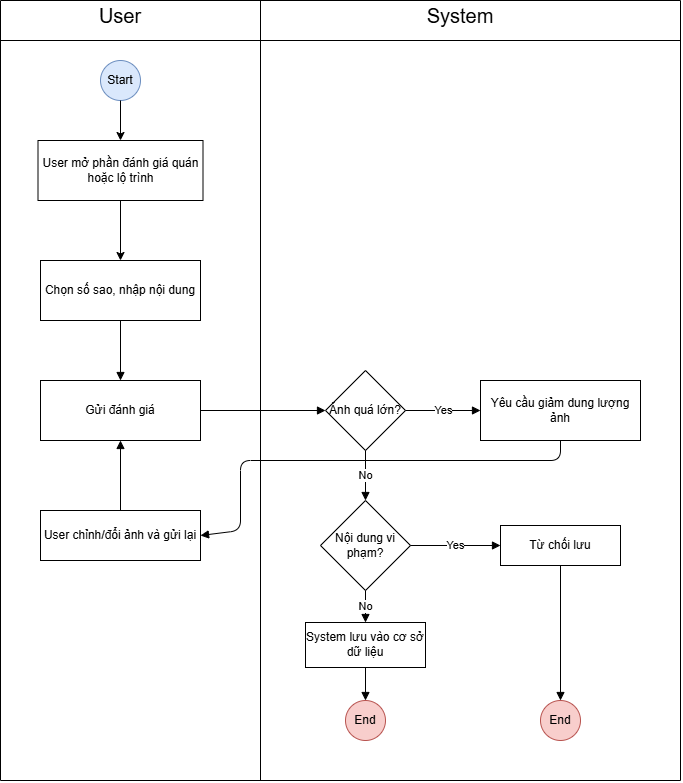
\includegraphics[width=0.9\textwidth]{img/activity/Activity_Danh_Gia.drawio.png}
    \caption{Activity Diagram Review}
\end{figure}

Hình 4.3 minh họa biểu đồ hoạt động cho chức năng đăng nhập và đăng xuất của hệ thống. Biểu đồ thể hiện quá trình người dùng nhập thông tin xác thực, hệ thống kiểm tra tính hợp lệ và trạng thái tài khoản, từ đó cho phép đăng nhập, thông báo lỗi hoặc kết thúc phiên làm việc khi người dùng đăng xuất.

\begin{figure}[H]
    \centering
    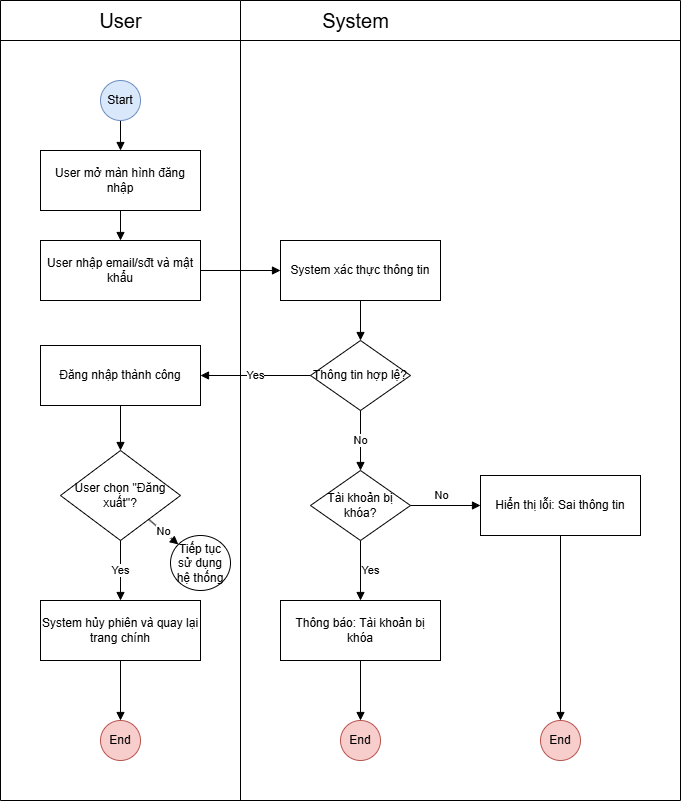
\includegraphics[width=0.9\textwidth]{img/activity/Activity_Diagram_Login_Logout.drawio.png}
    \caption{Activity Diagram Login Logout}
\end{figure}

Hình 4.4 minh họa biểu đồ hoạt động cho chức năng tìm kiếm và tra cứu thông tin quán ăn. Biểu đồ mô tả quá trình người dùng nhập từ khóa hoặc chọn khu vực tìm kiếm, hệ thống trả về kết quả tương ứng, đồng thời hỗ trợ xem chi tiết quán ăn và lưu quán yêu thích khi có nhu cầu.

\begin{figure}[H]
    \centering
    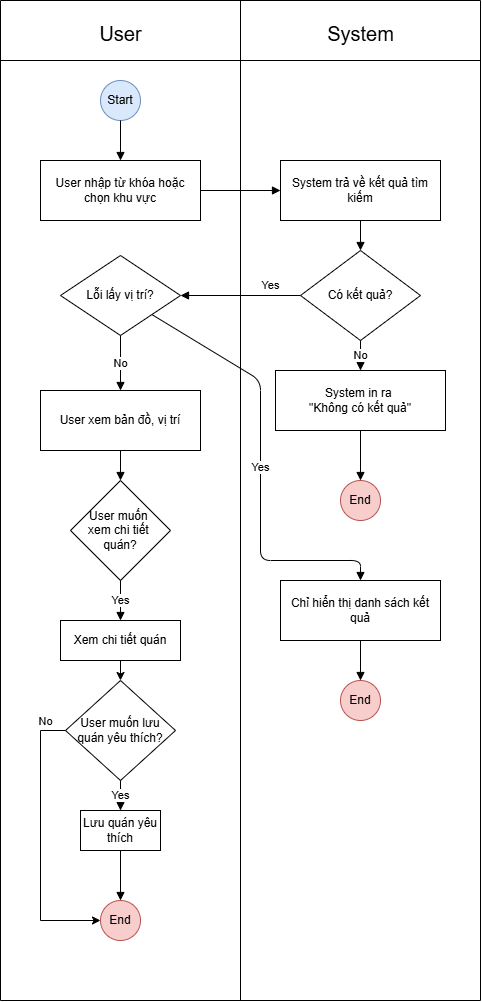
\includegraphics[width=0.68\textwidth]{img/activity/Activity_Find_Restaurant.drawio.png}
    \caption{Activity Diagram Search Restaurant}
\end{figure}

Hình 4.5 minh họa biểu đồ hoạt động cho chức năng tối ưu lộ trình food tour. Biểu đồ thể hiện quá trình người dùng lựa chọn các quán ăn, hệ thống tính toán lộ trình di chuyển phù hợp, hiển thị kết quả hoặc đề xuất phương án thay thế, đồng thời cho phép người dùng lưu, chỉnh sửa hoặc đánh giá lộ trình.

\begin{figure}[H]
    \centering
    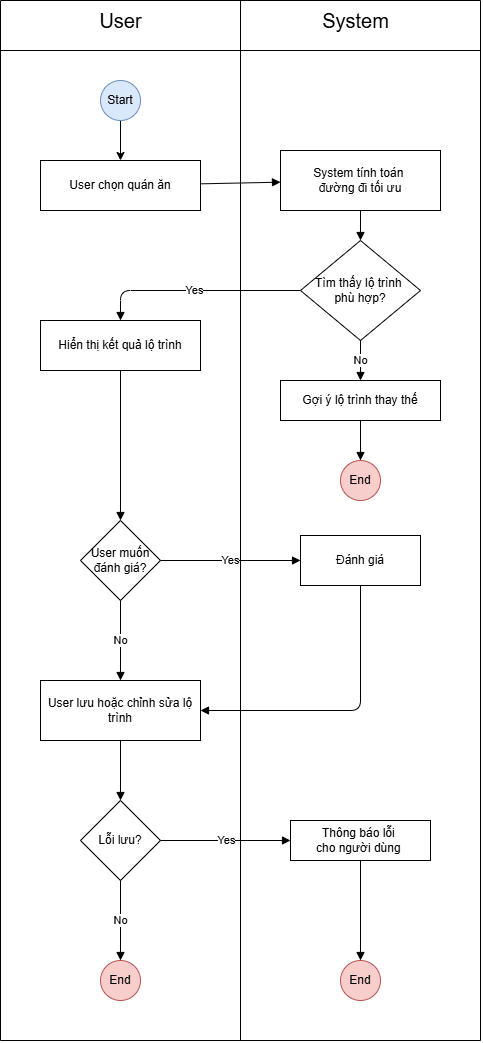
\includegraphics[width=0.57\textwidth]{img/activity/Activity_Find_Route.png}
    \caption{Activity Diagram Food Tour}
\end{figure}

Hình 4.6 minh họa biểu đồ hoạt động cho chức năng cập nhật hồ sơ cá nhân của người dùng. Biểu đồ thể hiện quá trình người dùng chỉnh sửa thông tin cá nhân, hệ thống kiểm tra và lưu dữ liệu, đồng thời cập nhật cơ chế gợi ý cá nhân hóa khi thông tin hợp lệ.

\begin{figure}[H]
    \centering
    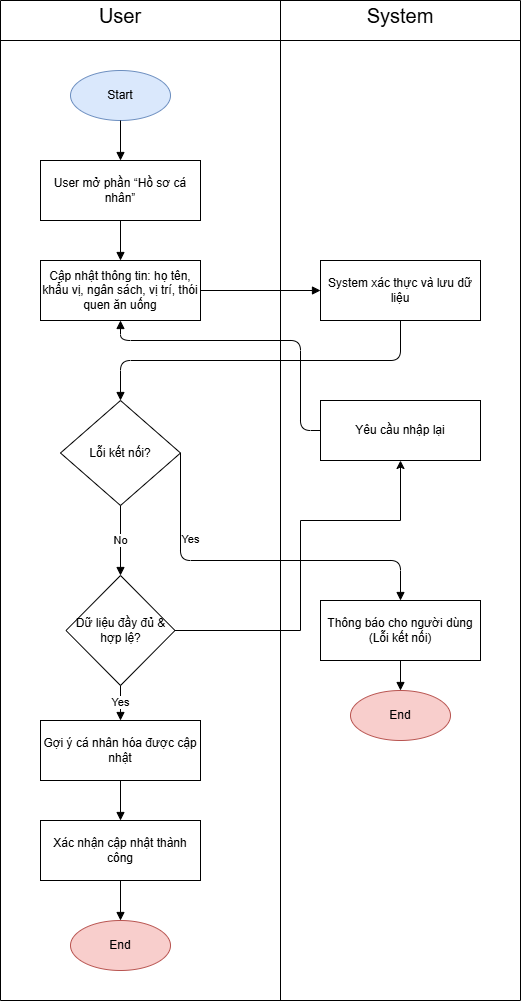
\includegraphics[width=0.57\textwidth]{img/activity/Activity_User_Profile_Edit.drawio.png}
    \caption{Activity Diagram Edit Profile}
\end{figure}
\newpage
Hình 4.7 minh họa biểu đồ hoạt động cho chức năng quản lý dữ liệu quán ăn của quản trị viên. Biểu đồ thể hiện quy trình admin thực hiện các thao tác thêm, sửa hoặc xóa thông tin quán ăn, trong đó hệ thống kiểm tra tính hợp lệ của dữ liệu và xử lý các trường hợp lỗi trước khi cập nhật thông tin cho người dùng.

\begin{figure}[H]
    \centering
    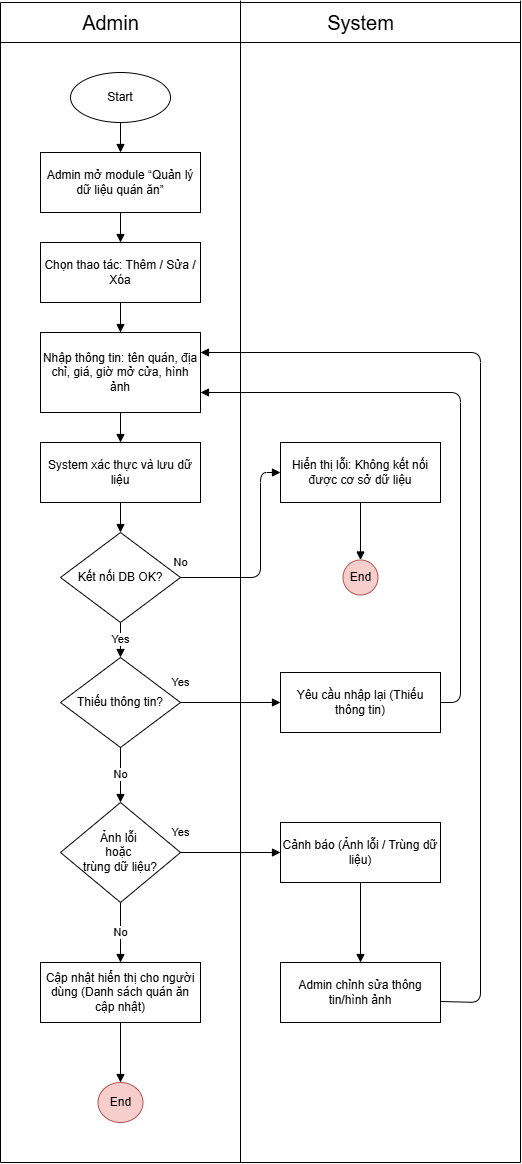
\includegraphics[width=0.57\textwidth]{img/activity/Activity_Quan_Ly_Du_Lieu_Quan_An.drawio.png}
    \caption{Activity Diagram CUD Restaurant by Admin}
\end{figure}

Hình 4.8 minh họa biểu đồ hoạt động cho chức năng quản lý tài khoản người dùng của quản trị viên. Biểu đồ thể hiện quy trình admin tìm kiếm tài khoản, xem thông tin chi tiết và thực hiện các thao tác khóa hoặc mở khóa, đồng thời hệ thống xử lý việc lưu trữ thay đổi và thông báo kết quả tương ứng.

\begin{figure}[H]
    \centering
    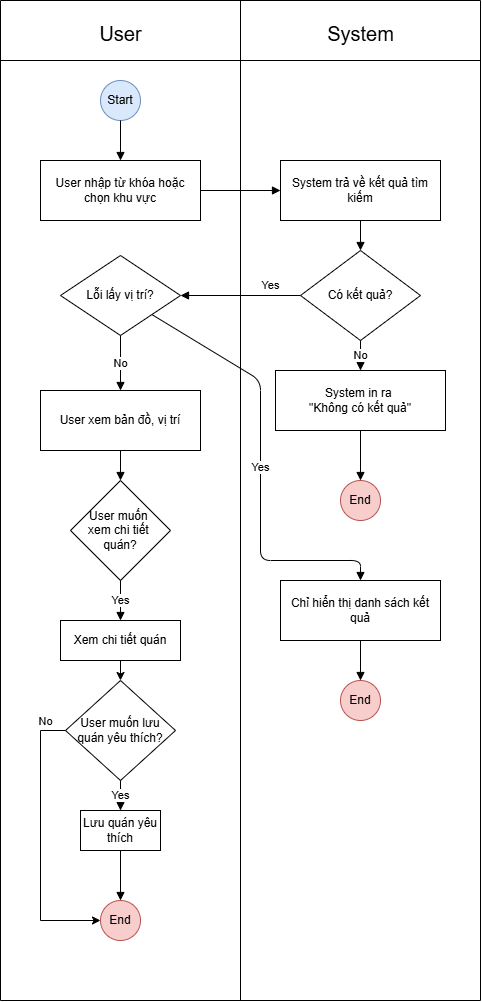
\includegraphics[width=0.57\textwidth]{img/activity/Activity_Find_Restaurant.drawio.png}
    \caption{Activity Diagram Lock/UnLock Account by Admin}
\end{figure}


\subsection{Sequence Diagram }
Sau khi mô tả luồng xử lý nghiệp vụ thông qua các biểu đồ hoạt động, luận văn tiếp tục sử dụng biểu đồ tuần tự (Sequence Diagram) nhằm làm rõ sự tương tác giữa các đối tượng trong hệ thống theo trục thời gian khi thực hiện từng chức năng cụ thể. Biểu đồ tuần tự giúp thể hiện rõ thứ tự các thông điệp được trao đổi giữa người dùng, các thành phần giao diện và các lớp xử lý nghiệp vụ, từ đó làm rõ cách hệ thống phối hợp để hoàn thành một kịch bản sử dụng.

Trong mục này, các biểu đồ tuần tự được xây dựng cho những chức năng tiêu biểu của hệ thống, qua đó minh họa chi tiết quá trình xử lý từ thời điểm người dùng khởi tạo yêu cầu cho đến khi hệ thống phản hồi kết quả tương ứng.


Hình 4.9 minh họa biểu đồ tuần tự cho chức năng quản lý tài khoản người dùng của quản trị viên. Biểu đồ thể hiện trình tự tương tác giữa admin, giao diện quản trị, dịch vụ xử lý và cơ sở dữ liệu trong quá trình tìm kiếm người dùng và thực hiện thao tác khóa hoặc mở khóa tài khoản.

\begin{figure}[H]
    \centering
    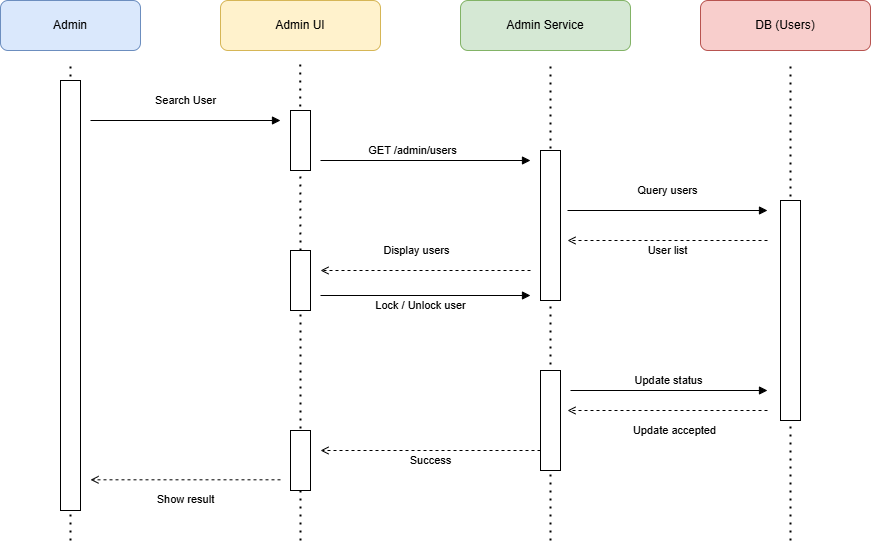
\includegraphics[width=1\textwidth]{img/sequence/Sequence_Account_Management.drawio.png}
    \caption{Sequence Diagram Account Management by Admin}
\end{figure}

Hình 4.10 minh họa biểu đồ tuần tự cho chức năng tạo và hiển thị lịch trình ăn uống. Biểu đồ thể hiện trình tự tương tác giữa người dùng, giao diện ứng dụng, dịch vụ xử lý và API bản đồ trong quá trình tạo lộ trình và trả về thông tin di chuyển tương ứng.

\begin{figure}[H]
    \centering
    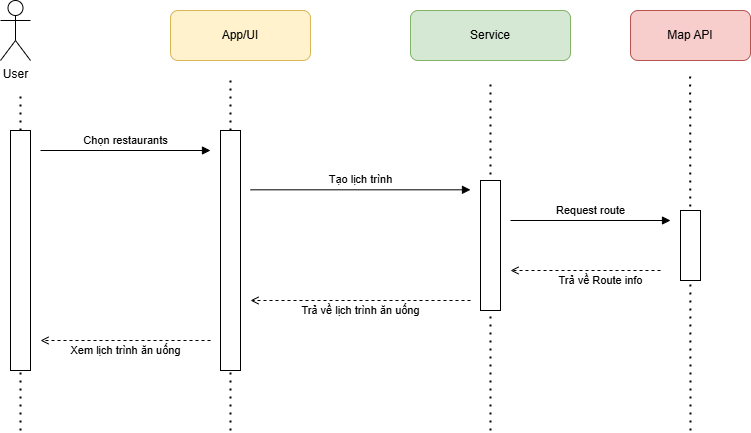
\includegraphics[width=1\textwidth]{img/sequence/Sequence_Create_Foot_Route.drawio.png}
    \caption{Sequence Diagram Create Food Tour}
\end{figure}

Hình 4.11 minh họa biểu đồ tuần tự cho chức năng tạo và lưu đánh giá quán ăn. Biểu đồ thể hiện trình tự tương tác giữa người dùng, giao diện ứng dụng, dịch vụ đánh giá và cơ sở dữ liệu trong quá trình gửi, lưu trữ và hiển thị nội dung đánh giá.

\begin{figure}[H]
    \centering
    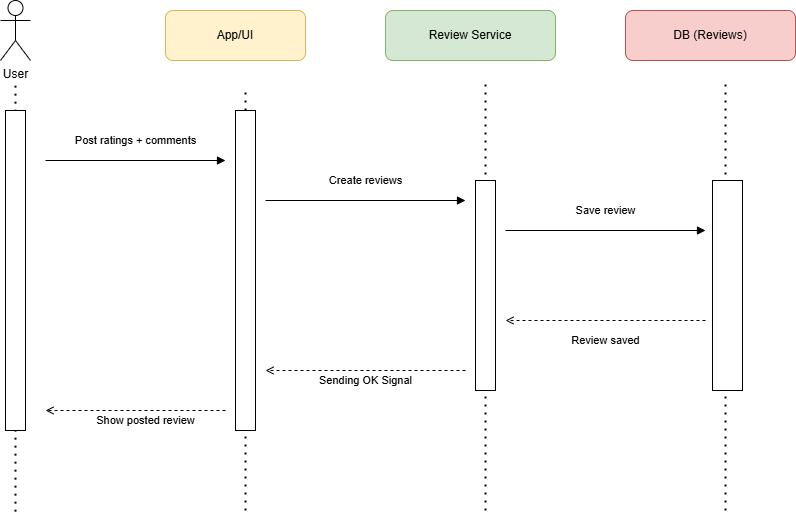
\includegraphics[width=0.92\textwidth]{img/sequence/Sequence_Danh_Gia.drawio.png}
    \caption{Sequence Diagram Review}
\end{figure}

Hình 4.12 minh họa biểu đồ tuần tự cho chức năng đăng nhập hệ thống. Biểu đồ thể hiện trình tự tương tác giữa người dùng, giao diện ứng dụng, dịch vụ xác thực và cơ sở dữ liệu trong quá trình kiểm tra thông tin đăng nhập và trả về kết quả xác thực.

\begin{figure}[H]
    \centering
    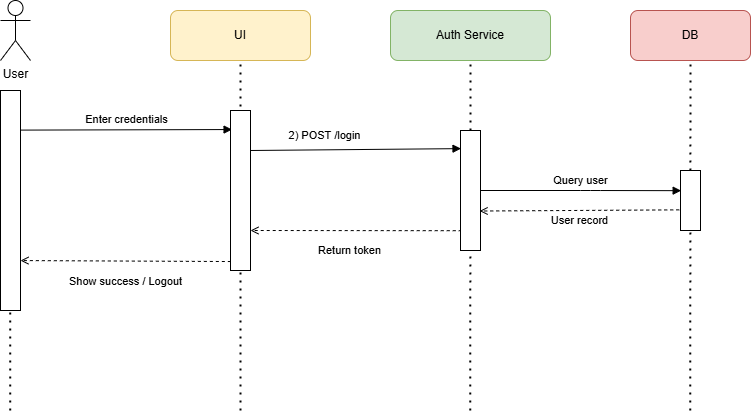
\includegraphics[width=1\textwidth]{img/sequence/Sequence_Login.drawio.png}
    \caption{Sequence Diagram Login}
\end{figure}

Hình 4.13 minh họa biểu đồ tuần tự cho chức năng quản lý thông tin quán ăn của quản trị viên. Biểu đồ thể hiện trình tự tương tác giữa admin, giao diện quản trị, dịch vụ quản lý quán ăn và cơ sở dữ liệu trong quá trình thêm, chỉnh sửa hoặc xóa thông tin quán ăn.

\begin{figure}[H]
    \centering
    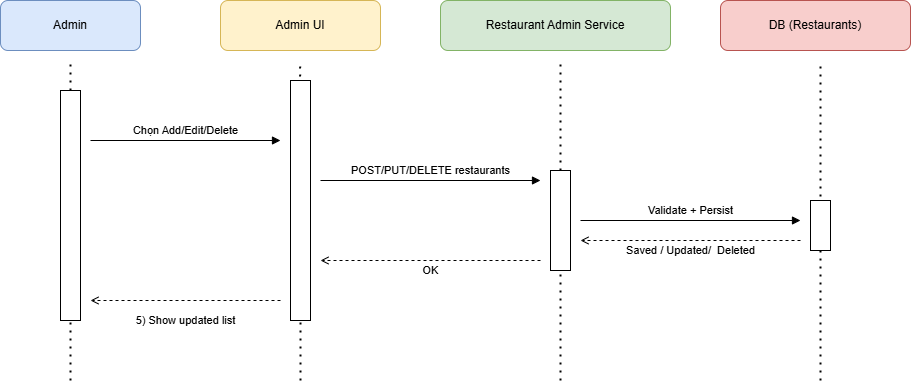
\includegraphics[width=1\textwidth]{img/sequence/Sequence_Restaurant_Data_Management.drawio.png}
    \caption{Sequence Diagram Restaurant Management by Admin}
\end{figure}

Hình 4.14 minh họa biểu đồ tuần tự cho chức năng tìm kiếm và lọc quán ăn. Biểu đồ thể hiện trình tự tương tác giữa người dùng, giao diện ứng dụng, dịch vụ tìm kiếm và cơ sở dữ liệu trong quá trình truy vấn và trả về danh sách kết quả phù hợp.

\begin{figure}[H]
    \centering
    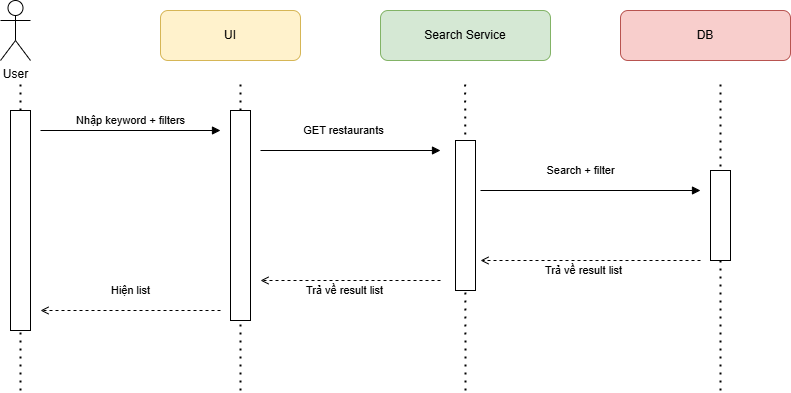
\includegraphics[width=1\textwidth]{img/sequence/Sequence_Search_Restaurant.drawio.png}
    \caption{Sequence Diagram Search Restaurant}
\end{figure}


Hình 4.15 minh họa biểu đồ tuần tự cho chức năng xem và cập nhật hồ sơ cá nhân của người dùng. Biểu đồ thể hiện trình tự tương tác giữa người dùng, giao diện ứng dụng, dịch vụ người dùng và cơ sở dữ liệu trong quá trình truy xuất và cập nhật thông tin hồ sơ.

\begin{figure}[H]
    \centering
    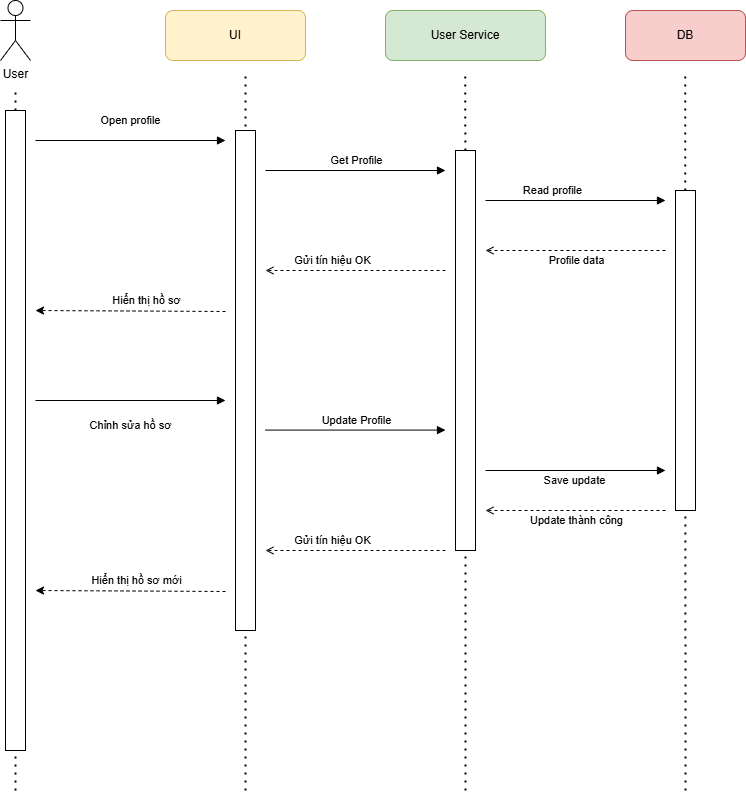
\includegraphics[width=1\textwidth]{img/sequence/Sequence_User_Profile_Edit.drawio.png}
    \caption{Sequence Diagram Edit Profile}
\end{figure}



\subsection{Class Diagram }

Biểu đồ lớp (Class Diagram) được sử dụng để mô tả cấu trúc tĩnh của hệ thống FoodTour Planner thông qua việc xác định các lớp chính, thuộc tính, phương thức và mối quan hệ giữa các lớp. Mục tiêu của biểu đồ này là làm rõ cách hệ thống tổ chức dữ liệu và phân tách trách nhiệm giữa các thành phần, từ đó làm cơ sở cho quá trình hiện thực hóa các chức năng đã nêu trong phần yêu cầu.

Về mặt mô hình dữ liệu, hệ thống được xây dựng xoay quanh các lớp cốt lõi gồm User, Restaurant, FoodTour, FoodTourStop, Review và Cuisine. Trong đó, lớp User đại diện cho người dùng hệ thống, lưu trữ các thông tin định danh và xác thực (email/username/phone, password\_hash), cũng như các thông tin phục vụ cá nhân hóa như taste\_profile. Ngoài ra, người dùng có thể đánh dấu quán ăn yêu thích và lưu các food tour công khai để tham khảo, do đó lớp User có các thuộc tính danh sách như favorite\_restaurant\_ids và saved\_tour\_ids. Các phương thức của User tập trung vào các hành vi nghiệp vụ trực tiếp liên quan đến người dùng như đăng ký/đăng nhập, cập nhật hồ sơ, tạo đánh giá và tạo food tour.

Lớp Restaurant mô tả dữ liệu quán ăn/nhà hàng, bao gồm thông tin cơ bản (tên, địa chỉ, số điện thoại, mô tả, hình ảnh), thông tin phục vụ tìm kiếm/lọc (tags, pricerange), và thông tin giờ mở cửa. Trường avg\_rating được đánh dấu là thuộc tính suy diễn (derived), thể hiện giá trị tổng hợp từ các đánh giá trong lớp Review nhằm hỗ trợ hiển thị nhanh và sắp xếp theo mức độ đánh giá. Lớp Cuisine biểu diễn loại ẩm thực, và mối quan hệ giữa Restaurant và Cuisine được mô hình hóa dạng nhiều-nhiều (một quán có thể thuộc nhiều loại ẩm thực và một loại ẩm thực có thể có nhiều quán).

Đối với chức năng food tour, lớp FoodTour đại diện cho một hành trình ăn uống do người dùng tạo. FoodTour chứa các thông tin như tiêu đề, mô tả, trạng thái hiển thị visibility và tổng quãng đường total\_distance. Một food tour bao gồm nhiều điểm dừng, do đó lớp FoodTourStop được sử dụng như một lớp trung gian để liên kết giữa FoodTour và Restaurant, đồng thời lưu trữ thứ tự ghé thăm thông qua thuộc tính order\_index. Việc tách FoodTourStop giúp biểu diễn đúng nghiệp vụ “một quán có thể xuất hiện trong nhiều food tour” và “một food tour gồm nhiều quán theo thứ tự”, đồng thời hỗ trợ thao tác sắp xếp lại điểm dừng và tối ưu lộ trình.

Lớp Review biểu diễn đánh giá của người dùng đối với quán ăn, với các thuộc tính chính gồm user\_id, restaurant\_id, rating và content. Mối quan hệ giữa User và Review là 1–n (một người dùng có thể viết nhiều đánh giá), tương tự Restaurant và Review cũng là 1–n (một quán có nhiều đánh giá). Thiết kế này phù hợp với yêu cầu hiển thị danh sách đánh giá trong trang chi tiết quán ăn, đồng thời tạo nền tảng để tính toán trung bình đánh giá cho Restaurant.

Bên cạnh các lớp dữ liệu (entity), hệ thống có lớp AdminService nhằm thể hiện các chức năng quản trị như quản lý dữ liệu quán ăn (thêm/sửa/xóa), quản lý tài khoản người dùng (khóa/mở khóa) và kiểm duyệt nội dung food tour công khai. Việc đặt các hành vi quản trị trong lớp dịch vụ thay vì gắn trực tiếp vào lớp User nhằm đảm bảo nguyên tắc phân tách trách nhiệm và hỗ trợ kiểm soát phân quyền rõ ràng. 
\newpage
Hình 4.16 trình bày class diagram tổng quan của hệ thống theo các nhóm lớp nêu trên.
\begin{figure}[H]
    \centering
    \includegraphics[page=1,width=1\textwidth]{img/4.png}
    \caption{Class Diagram}
\end{figure}




